\documentclass[tikz,border=8pt]{standalone}

\usepackage{amsmath,amssymb}
\usetikzlibrary{arrows.meta,backgrounds,calc,fit,positioning}

\definecolor{mlpfill}{HTML}{B7CAE8}
\definecolor{mlpdraw}{HTML}{2459A6}
\definecolor{sumfill}{HTML}{FFE2CC}
\definecolor{sumdraw}{HTML}{D95F02}
\definecolor{geomfill}{HTML}{C9C7C7}
\definecolor{geomdraw}{HTML}{4D4D4D}
\definecolor{groupdraw}{HTML}{9B9B9B}

\begin{document}
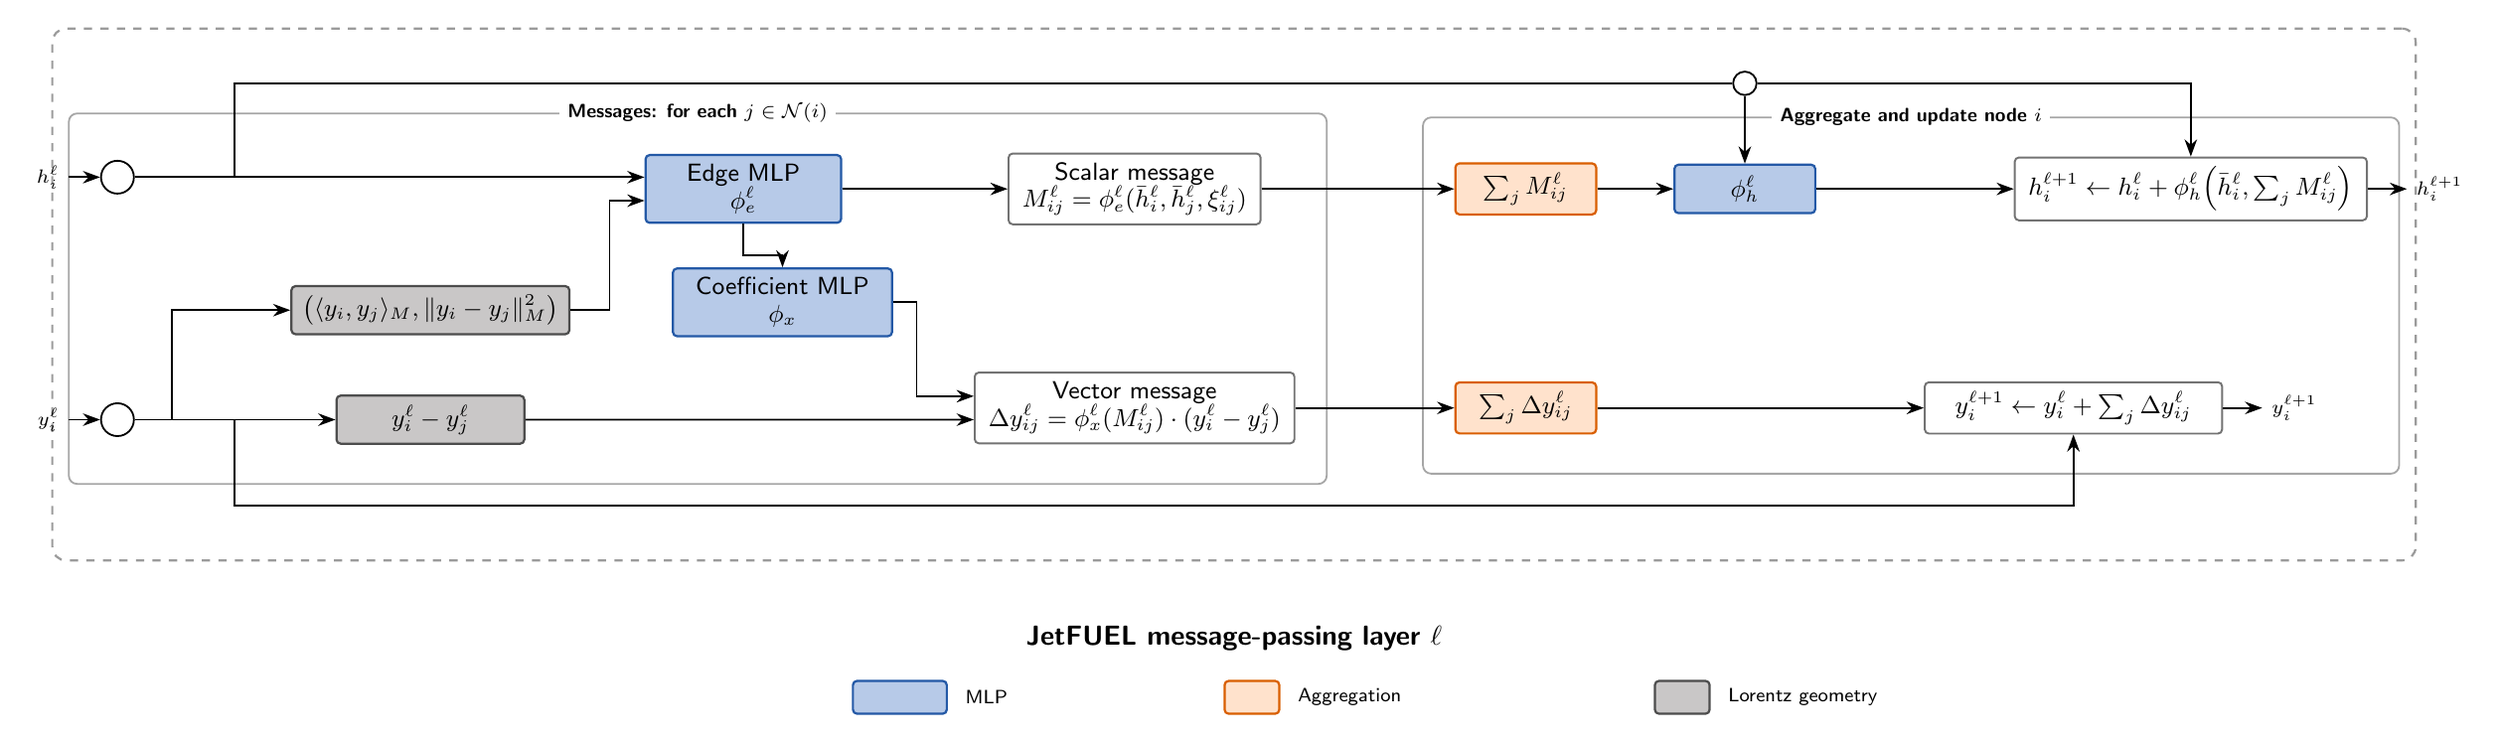
\begin{tikzpicture}[
  font=\sffamily\small,
  >={Stealth[length=2.2mm,width=1.6mm]},
  signal/.style={->, draw=black, line width=0.65pt},
  wire/.style={draw=black, line width=0.65pt},
  mlp/.style={
    draw=mlpdraw, fill=mlpfill, line width=0.8pt,
    rounded corners=1.5pt, minimum height=6.2mm,
    minimum width=25mm, align=center, inner xsep=5pt
  },
  sum/.style={
    draw=sumdraw, fill=sumfill, line width=0.8pt,
    rounded corners=1.5pt, minimum height=5.6mm,
    minimum width=18mm, align=center, inner xsep=4pt
  },
  geometry/.style={
    draw=geomdraw, fill=geomfill, line width=0.8pt,
    rounded corners=1.5pt, minimum height=5.6mm,
    minimum width=18mm, align=center, inner xsep=4pt
  },
  result/.style={
    draw=black!55, fill=white, line width=0.7pt,
    rounded corners=1.5pt, minimum height=5.8mm,
    minimum width=20mm, align=center, inner xsep=5pt
  },
  junction/.style={
    circle, draw=black, fill=white, line width=0.65pt,
    minimum size=4.2mm, inner sep=0pt, font=\scriptsize
  },
  annotation/.style={font=\sffamily\scriptsize, align=center},
  title/.style={font=\sffamily\bfseries, align=center}
]

% Inputs to one message-passing layer.
\node[junction] (jH) at (2, 1.5) {};
\node[junction] (jY) at (2, -1.6) {};
\node[annotation, left=4mm of jH] (inputH) {$h_i^\ell$};
\node[annotation, left=4mm of jY] (inputY) {$y_i^\ell$};
\draw[signal] (inputH.east) -- (jH.west);
\draw[signal] (inputY.east) -- (jY.west);

% Construct scalar and vector messages for every neighbor j.
\node[geometry] (invariants) at (6.0, -0.2)
  {$\left(\langle y_i,y_j\rangle_M,\|y_i-y_j\|_M^2\right)$};
\node[geometry, minimum width=24mm] (displacement) at (6.0, -1.6)
  {$y_i^\ell-y_j^\ell$};

\node[mlp, minimum width=25mm] (edgeMlp) at (10.0, 1.35)
  {Edge MLP\\[-1pt]$\phi_e^\ell$};
\node[mlp, minimum width=28mm] (vectorMlp) at (10.5, -0.1)
  {Coefficient MLP\\[-1pt]$\phi_x$};

\node[result, minimum width=18mm] (scalarMessage) at (15.0, 1.35)
  {Scalar message\\[-1pt]
   $M_{ij}^\ell=\phi_e^\ell(\bar h_i^\ell,\bar h_j^\ell,\xi_{ij}^\ell)$};
\node[result, minimum width=33mm] (vectorMessage) at (15.0, -1.45)
  {Vector message\\[-1pt]
   $\Delta y_{ij}^\ell=\phi_x^\ell(M_{ij}^\ell)\cdot(y_i^\ell-y_j^\ell)$};

% Aggregate the two message types and apply residual updates.
\node[sum] (sumH) at (20.0, 1.35) {$\sum_j M_{ij}^\ell$};
\node[mlp, minimum width=18mm] (scalarMlp) at (22.8, 1.35) {$\phi_h^\ell$};
\node[result, minimum width=34mm] (updateH) at (28.5, 1.35)
  {$h_i^{\ell+1}\leftarrow h_i^\ell+
    \phi_h^\ell\!\left(\bar h_i^\ell,\sum_jM_{ij}^\ell\right)$};

\node[sum] (sumY) at (20.0, -1.45) {$\sum_j\Delta y_{ij}^\ell$};
\node[result, minimum width=38mm] (updateY) at (27.0, -1.45)
  {$y_i^{\ell+1}\leftarrow y_i^\ell+\sum_j\Delta y_{ij}^\ell$};

% Message inputs and construction.
\draw[signal] (jH) -- ($(edgeMlp.west)+(0,0.15)$);
\draw[signal] (jY) -- (displacement.west);
\draw[signal] (jY) -- ++(0.7,0) |- (invariants.west);
\draw[signal] (invariants.east) -- ++(0.5,0)
  |- ($(edgeMlp.west)+(0,-0.15)$);
\draw[signal] (edgeMlp.east) -- (scalarMessage.west);
\draw[signal] (edgeMlp.south) -- ++(0,-0.4) -| (vectorMlp.north);
\draw[signal] (vectorMlp.east) -- ++(0.3,0)
  |- ($(vectorMessage.west)+(0,0.15)$);
\draw[signal] (displacement.east)
  -- ($(vectorMessage.west)+(0,-0.15)$);

% Aggregation and updates.
\draw[signal] (scalarMessage.east) -- (sumH.west);
\draw[signal] (sumH.east) -- (scalarMlp.west);
\draw[signal] (scalarMlp.east) -- (updateH.west);
\draw[signal] (vectorMessage.east) -- (sumY.west);
\draw[signal] (sumY.east) -- (updateY.west);

% Orthogonal residual bypasses.
\node[junction, minimum size=3mm] (residualFork) at (22.8, 2.7) {};
\draw[wire] (jH) -- (3.5,1.5) -- (3.5,2.7) -- (residualFork.west);
\draw[signal] (residualFork.south) -- (scalarMlp.north);
\draw[signal] (residualFork.east) -- (28.5,2.7) -- (updateH.north);
\draw[signal] (jY) -- (3.5,-1.6) -- (3.5,-2.7)
  -- (27.0,-2.7) -- (updateY.south);

% Output labels.
\node[annotation, right=5mm of updateH] (outputH) {$h_i^{\ell+1}$};
\node[annotation, right=5mm of updateY] (outputY) {$y_i^{\ell+1}$};
\draw[signal] (updateH.east) -- (outputH.west);
\draw[signal] (updateY.east) -- (outputY.west);

% Substage and layer boundaries.
\coordinate (bypassH_NW) at (2.8,3.2);
\coordinate (bypassH_NE) at (31.0,3.2);
\coordinate (bypassY_SW) at (2.8,-3.2);
\coordinate (bypassY_SE) at (31.0,-3.2);
\begin{scope}[on background layer]
  \node[
    draw=black!35, line width=0.65pt, rounded corners=3pt,
    fit=(jH)(jY)(invariants)(edgeMlp)(scalarMessage)
        (vectorMlp)(displacement)(vectorMessage),
    inner xsep=4mm, inner ysep=5mm
  ] (messageGroup) {};
  \node[
    draw=black!35, line width=0.65pt, rounded corners=3pt,
    fit=(sumH)(scalarMlp)(sumY)(updateH)(updateY),
    inner xsep=4mm, inner ysep=5mm
  ] (updateGroup) {};
  \node[
    draw=groupdraw, dashed, line width=0.8pt, rounded corners=5pt,
    fit=(bypassH_NW)(bypassY_SW)(bypassH_NE)(bypassY_SE)
        (messageGroup)(updateGroup),
    inner xsep=2mm, inner ysep=2mm
  ] (layerGroup) {};
\end{scope}

\node[annotation, font=\sffamily\scriptsize\bfseries,
      fill=white, inner xsep=3pt]
  at (messageGroup.north) {Messages: for each $j\in\mathcal N(i)$};
\node[annotation, font=\sffamily\scriptsize\bfseries,
      fill=white, inner xsep=3pt]
  at (updateGroup.north) {Aggregate and update node $i$};

\node[title, below=7mm of layerGroup] (figureTitle)
  {JetFUEL message-passing layer $\ell$};

% Operation legend.
\node[mlp, minimum width=12mm, minimum height=4.2mm]
  (legendMlp) at (12.0,-5.15) {};
\node[annotation, right=1mm of legendMlp] {MLP};
\node[sum, minimum width=7mm, minimum height=4.2mm]
  (legendSum) at (16.5,-5.15) {};
\node[annotation, right=1mm of legendSum] {Aggregation};
\node[geometry, minimum width=7mm, minimum height=4.2mm]
  (legendGeom) at (22.0,-5.15) {};
\node[annotation, right=1mm of legendGeom] {Lorentz geometry};

\end{tikzpicture}
\end{document}
